% ============================================================================
\section{Surface relaxation as a boundary-local-time estimator}
\label{sec:app:estimator}
% ============================================================================

The wall-counting of Sec.~\ref{sec:methods:mc} is a Monte-Carlo realisation of the
Brownstein--Tarr Robin boundary condition $D\,\partial_n M = -\rho\,M$
\citep{Brownstein1979}. That boundary condition is not a per-collision penalty: it is a
continuous absorbing wall, and its stochastic representation is the \emph{boundary local
time} $\mathcal L_{\partial\Omega}$ of reflected Brownian motion --- the (measure-theoretic)
contact the walker accumulates at the surface --- through the Feynman--Kac survival weight
$\exp(-\tfrac{\rho}{D}\,\mathcal L_{\partial\Omega})$ \citep{Grebenkov2007}. Any faithful
simulator therefore only has to \emph{estimate} $\mathcal L_{\partial\Omega}$ from the discrete
walk; different estimators agree in the $\Delta t\!\to\!0$ limit but differ at finite step.

We use the \emph{realised-overshoot} estimator: a step that crosses the wall contributes
$2\,d_\perp$ to $\mathcal L_{\partial\Omega}$, with $d_\perp$ the perpendicular overshoot of
that step, so the transverse magnetisation is scaled by $\exp(-2\rho\,d_\perp/D)$ per
encounter --- a \emph{pathwise} estimator weighted by the actual penetration depth. An
alternative, used by the multi-modal simulator \textsc{MCMRSimulator} (v1.0.0) of
\citet{Cottaar2025}, assigns every detected collision the \emph{same} cost
$\exp(-x\sqrt{\Delta t})$ (\texttt{src/evolve.jl}, lines 566--570), i.e.\ it replaces the per-step
penetration with its mean; its documented material rate is $x=\rho\sqrt{\pi/D}$, which we use
as given (no calibration). Both are legitimate; they differ only in whether the collision cost
carries the realised depth or a fixed $\sqrt{\Delta t}$.

To isolate the \emph{estimator} --- rather than two codebases, which would confound the
per-collision rule with stepping, detection and RNG --- we run one reflecting walk in a cylinder
cross-section ($R=3\,\mu$m, $D=3\,\mu$m$^2$/ms) and accumulate \emph{both} penalties on the
\emph{same} collisions, referenced to the exact lowest Robin eigenvalue (the root of
$(kR)J_1(kR)/J_0(kR)=\rho R/D$, of which the textbook $\rho\,(2/R)$ is only the
$\rho R/D\!\to\!0$ limit, larger by $\rho R/4D$). This is an \emph{estimator} comparison inside
one code, not a two-codebase cross-validation: reimplementing the fixed-$\sqrt{\Delta t}$ rule on
our own walk holds the stepping, detection and RNG common, so the only independent reference is
the exact Robin eigenvalue --- and it is against that eigenvalue, not against either simulator,
that correctness is judged. Both schemes reproduce it at a fine step
(Fig.~\ref{fig:app:estimator}B,C), confirming our surface term is implemented correctly; the
$\sqrt{\Delta t}$ rule being MCMRSimulator's documented choice, this also shows the two are
consistent in the fine-step limit, but it is not an agreement between two independent codes. We
adopt the realised-overshoot form (the factor $2$ is the local-time normalisation, nothing
fitted) because it is parameter-free and holds at coarser steps, where the fixed-$\sqrt{\Delta t}$
rule drifts to $-8\%$.

The estimator's relative error is a function of the two dimensionless groups $\rho R/D$ and
step$/R$ alone, so the accuracy shown at $R=3\,\mu$m transfers to any calibre: holding both
groups fixed and sweeping the radius from $3$ down to $0.1\,\mu$m leaves the error flat at
$-0.01\%$ (a scale-invariance check in the same script). This is what licenses carrying the
interior rate to the sub-micron calibres that dominate the bias --- they are not an
extrapolation but the \emph{same} dimensionless regime, and in fact an easier one: at the
physical $\rho$ a sub-micron axon has $\rho R/D\!\sim\!10^{-5}$, far deeper in fast diffusion
than the benchmark, where the estimator (and the Brownstein--Tarr rate itself) is most accurate
(panel~C).

\begin{figure}[t]
  \centering
  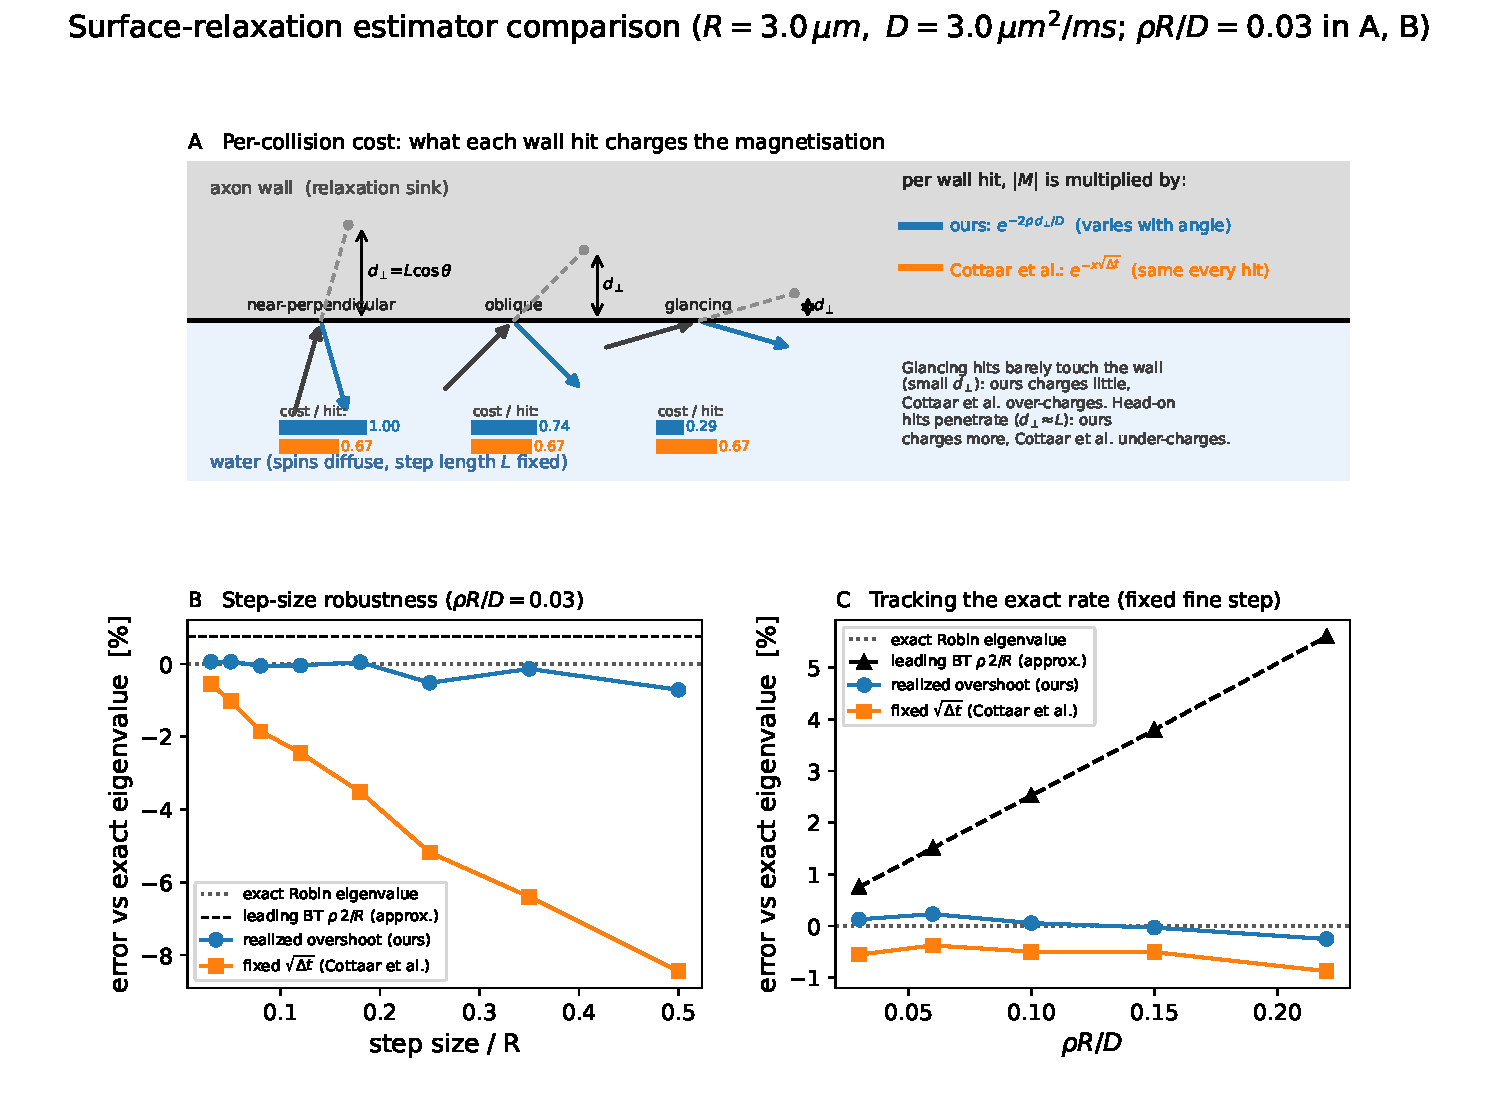
\includegraphics[width=\linewidth]{figures/appendix_estimator_comparison.pdf}
  \caption{Two Monte-Carlo estimators of the same Brownstein--Tarr surface relaxation, on
  identical collision events of one reflecting walk. \textbf{(A)} Per wall hit: for a fixed step
  $L$ the perpendicular overshoot $d_\perp=L\cos\theta$ grows from glancing to head-on, so the
  realised-overshoot rule charges $e^{-2\rho d_\perp/D}$ (blue, $1.00/0.74/0.29$) while the
  fixed-$\sqrt{\Delta t}$ rule charges the same each hit (orange, $0.67$) --- its mean over-charges
  glancing and under-charges head-on hits. \textbf{(B,C)} Error vs the exact Robin eigenvalue
  (dotted; leading $\rho(2/R)$ dashed): the parameter-free realised-overshoot estimator (ours)
  stays on the exact value across step size (B) and $\rho R/D$ (C); the fixed-$\sqrt{\Delta t}$
  rule (\citealp{Cottaar2025}) drifts to $-8\%$ at a coarse step (B); and the leading-order
  \emph{analytic} formula --- not the estimators --- diverges to $+5.6\%$ as $\rho R/D$ grows (C).}
  \label{fig:app:estimator}
\end{figure}

